\section{Представления}
В данном разделе создаётся представление по ранее созданной базе данных
предметной области «Геомониторинг автопарка каршеринга» и выполняются
запросы к нему.

\subsection*{Постановка задачи}
\begin{itemize}
	\item Создать представление на основе таблиц базы данных по предметной области Геомониторинг автопарка каршеринга.
	\item Написать и выполнить простой запрос к созданному представлению.
	\item Написать и выполнить сложный запрос к созданному представлению.
	% \item Проверить право доступа на изменение данных в представлении.
\end{itemize}

\subsection{Запрос для создание представления}
Для каждого автомобиля подсчитать количество тревожных событий и число парковочных зон, в которых этот автомобиль парковался.

\begin{lstlisting}[style=sqlstyle, caption={Создание представления \texttt{car\_stats}}, label={lst:view}]
CREATE VIEW car_stats AS
SELECT
	c.car_id,
	c.reg_number,
	COUNT(DISTINCT a.alert_event_id) AS alert_count,
	COUNT(DISTINCT pz.parking_zone_id) AS parking_count
FROM car c
LEFT JOIN alert_event a ON c.car_id = a.car_id
LEFT JOIN parking_session ps ON c.car_id = ps.car_id
LEFT JOIN parking_zone pz ON ps.parking_zone_id = pz.parking_zone_id
GROUP BY c.car_id, c.reg_number;
\end{lstlisting}

\begin{figure}[H]
    \centering
    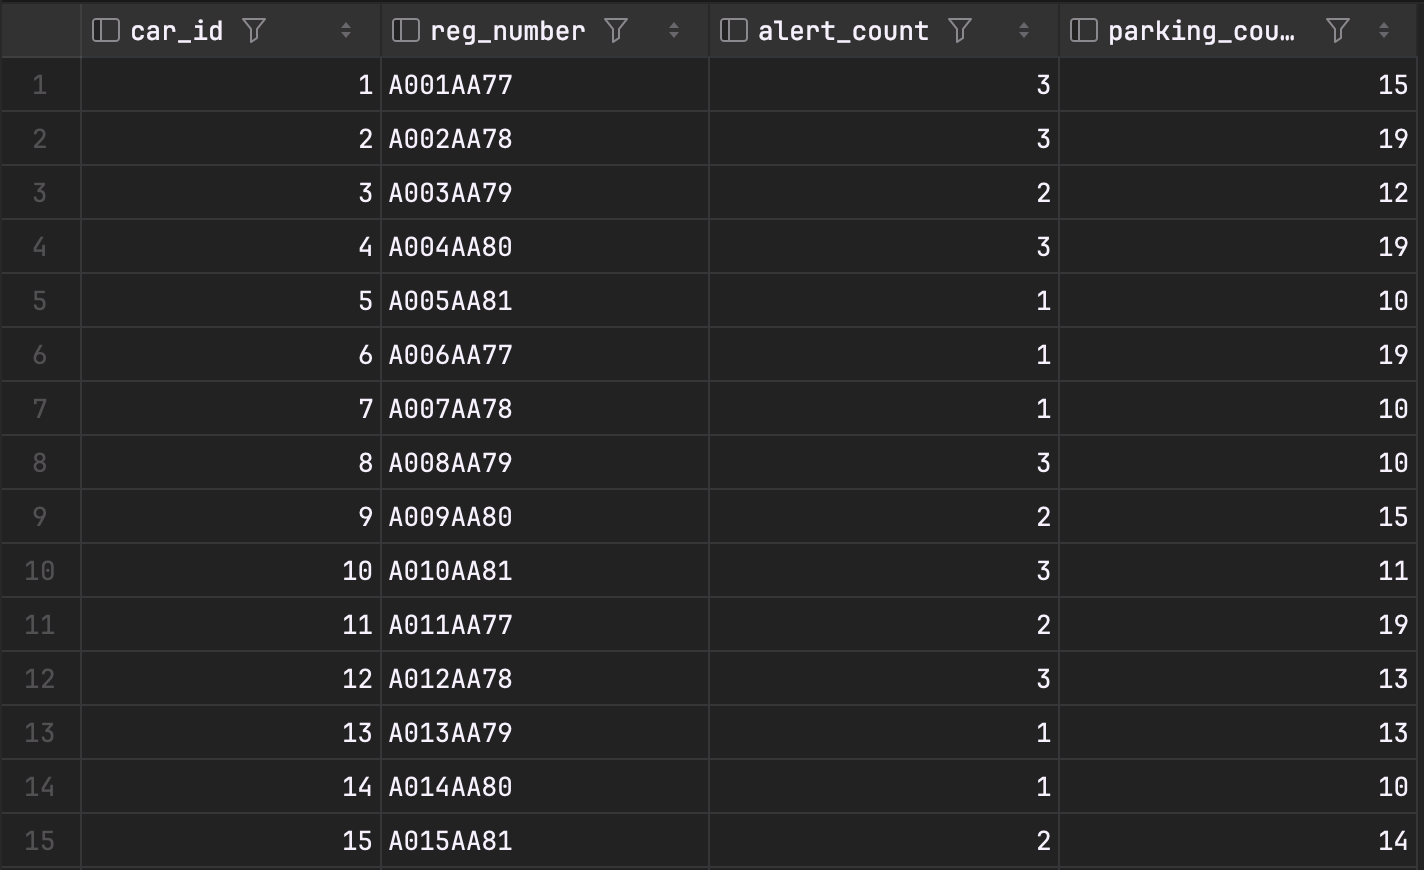
\includegraphics[width=0.5\linewidth]{myPhoto/view_result.png}
    \caption{Содержимое представления \texttt{car\_stats}}
    \label{fig:view_result}
\end{figure}

В качестве основной таблицы выбрана таблица \texttt{car}. \texttt{LEFT JOIN}
позволяют включить в представление каждый автомобиль, в том числе автомобиль
без тревожных событий и парковочных сессий. Использование
\texttt{COUNT(DISTINCT ...)} необходимо, поскольку соединение событий и
парковочных сессий может образовать повторяющиеся строки.

\noindent Реляционная формула представления:
\[
\begin{aligned}
&\gamma_{
  \substack{
    \text{car\_id},\;\text{reg\_number};\\
    \text{COUNT}(\text{alert\_event\_id}) \to \text{alert\_count};\\
    \text{COUNT}(\text{parking\_zone\_id}) \to \text{parking\_count}
  }
}\Bigl( \\
&\quad\text{car} \\
&\quad\bowtie(left)_{\,\text{car\_id}}\;\text{alert\_event} \\
&\quad\bowtie(left)_{\,\text{car\_id}}\;\text{parking\_session} \\
&\quad\bowtie(left)_{\,\text{parking\_zone\_id}}\;\text{parking\_zone} \\
&\Bigr)
\end{aligned}
\]

\subsection{Выполнение запросов к представлению}
\subsubsection*{Простой запрос}
Вывести автомобили, которые парковались более чем в N разных зонах и имеют хотя бы два тревожных события.

\begin{lstlisting}[style=sqlstyle, caption={Простой запрос}, label={lst:easy_query}]
SELECT
	c.reg_number,
	c.alert_count,
	c.parking_count
FROM
	car_stats c
WHERE
	c.parking_count > 17
	AND
	c.alert_count > 1;
\end{lstlisting}

Результат выполнения простого запроса представлен на
рисунке~\ref{fig:easy_query_result}.
\begin{figure}[H]
    \centering
    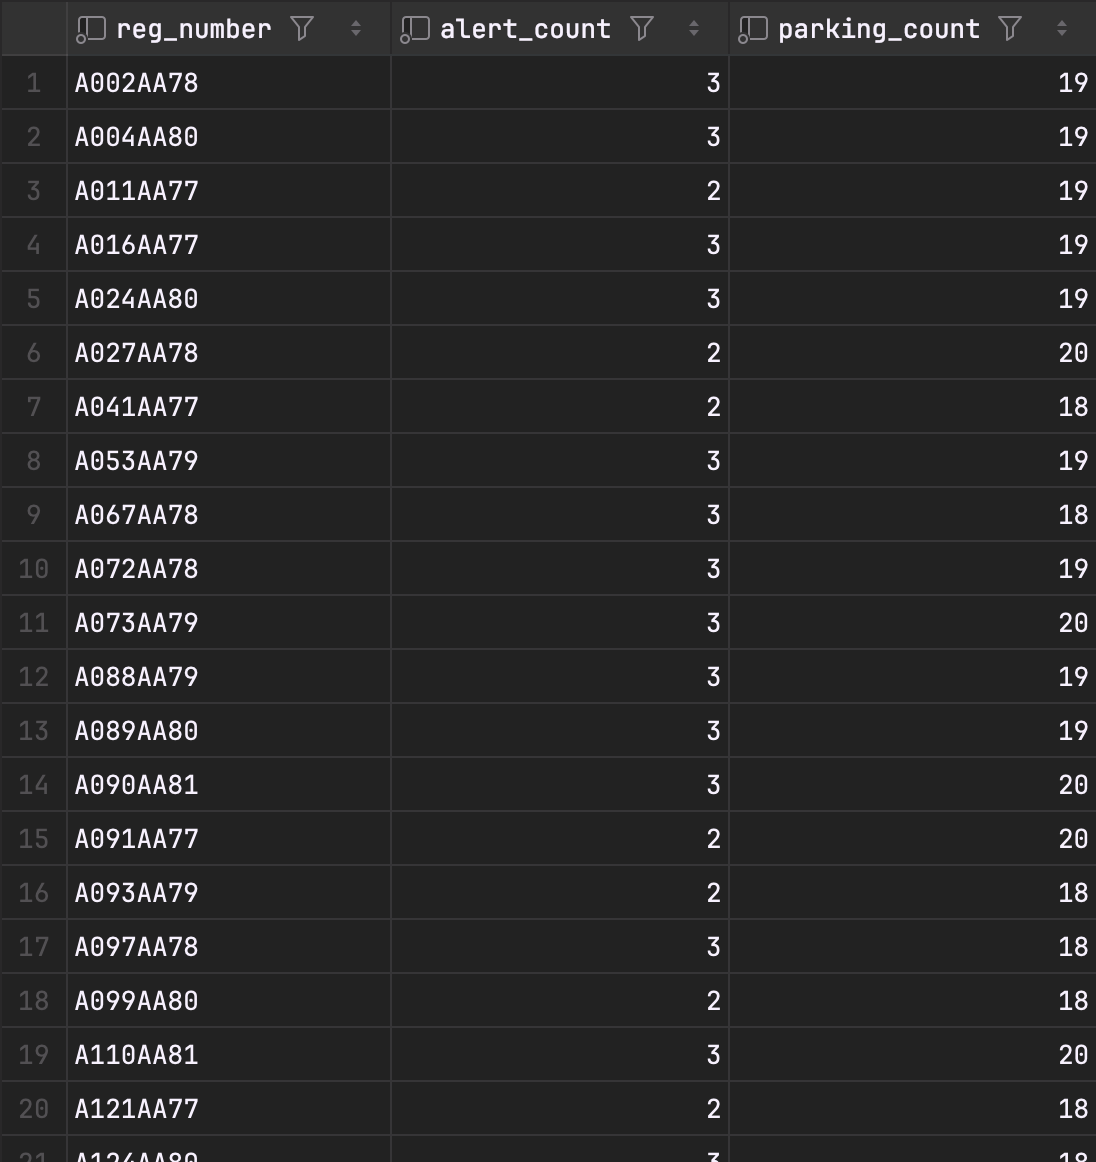
\includegraphics[width=0.5\linewidth]{myPhoto/easy_query_result.png}
    \caption{Результат выполнения простого запроса к представлению}
    \label{fig:easy_query_result}
\end{figure}

Время выполнения запроса: \\
Execution time: 0,207ms \\
Planning time: 0,291ms \\

\begin{figure}[H]
    \centering
    
\includegraphics[width=0.5\linewidth]{myPhoto/easy_explain.png}
    \caption{Последовательность выполнения простого запроса}
    \label{fig:easy_explain}
\end{figure}

\noindent Таблица \textbf{car\_stats} читается последовательно. Во время
чтения проверяются условия на количество парковочных зон и тревожных
событий, после чего в результат попадают только подходящие автомобили.

\noindent Реляционная формула запроса:
\[
\begin{aligned}
&\pi_{\text{reg\_number},\;\text{alert\_count},\;\text{parking\_count}}
\Bigl( \\
&\quad\sigma_{\text{parking\_count}>17\;\wedge\;\text{alert\_count}>1}
\Bigl( \\
&\qquad\text{car\_stats} \\
&\quad\Bigr) \\
&\Bigr)
\end{aligned}
\]



\subsubsection*{Сложный запрос}
Для выполнения сложного запроса к созданному представлению был сформулирован запрос: вывести автомобили, которые парковались менее чем в N разных зонах и имеют необработанные тревожные события заданного типа.

\begin{lstlisting}[style=sqlstyle, caption={Сложный запрос}, label={lst:hard_query}]
SELECT
	DISTINCT
	c.reg_number,
	c.alert_count
FROM
	car_stats c
JOIN
	alert_event a ON c.car_id = a.car_id
JOIN
	alert_event_process_status s ON a.status_id = s.status_id
JOIN
	alert_event_type t ON a.alert_event_type_id = t.alert_event_type_id
WHERE
	c.parking_count < 18
	AND 
	s.name = 'Новое'
	AND
	t.name = 'Потеря связи';
\end{lstlisting}

Результат выполнения сложного запроса представлен на
рисунке~\ref{fig:hard_query_result}. В результате выполнения было выведено
19 автомобилей.
\begin{figure}[H]
    \centering
    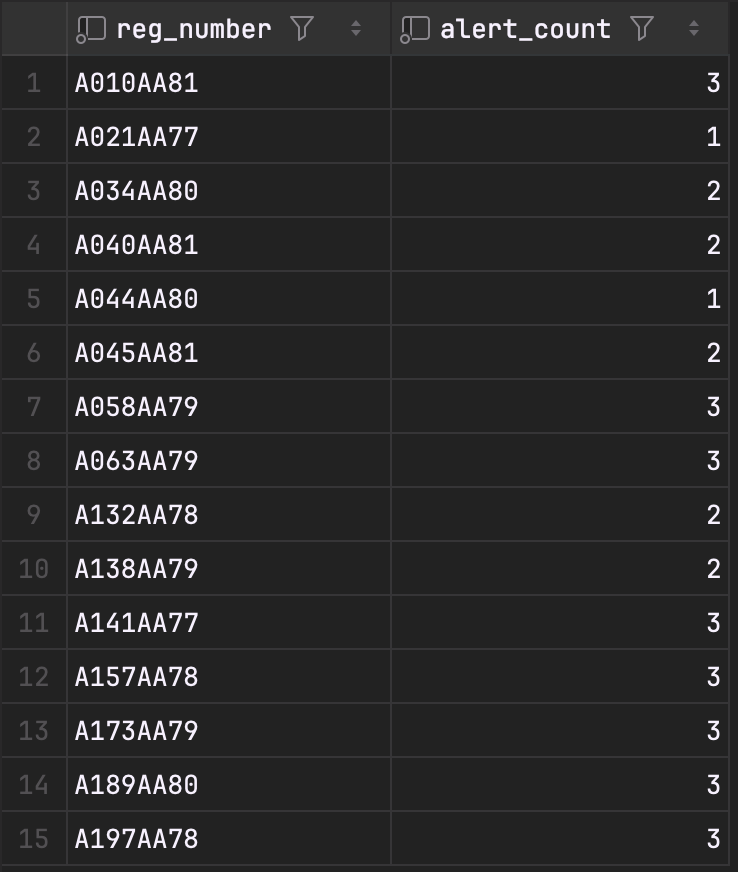
\includegraphics[width=0.5\linewidth]{myPhoto/hard_query_result.png}
    \caption{Результат выполнения сложного запроса к представлению}
    \label{fig:hard_query_result}
\end{figure}

Время выполнения запроса: \\
Execution time: 0,564ms \\ 
Planning time: 1,5ms \\

\begin{figure}[H]
    \centering
    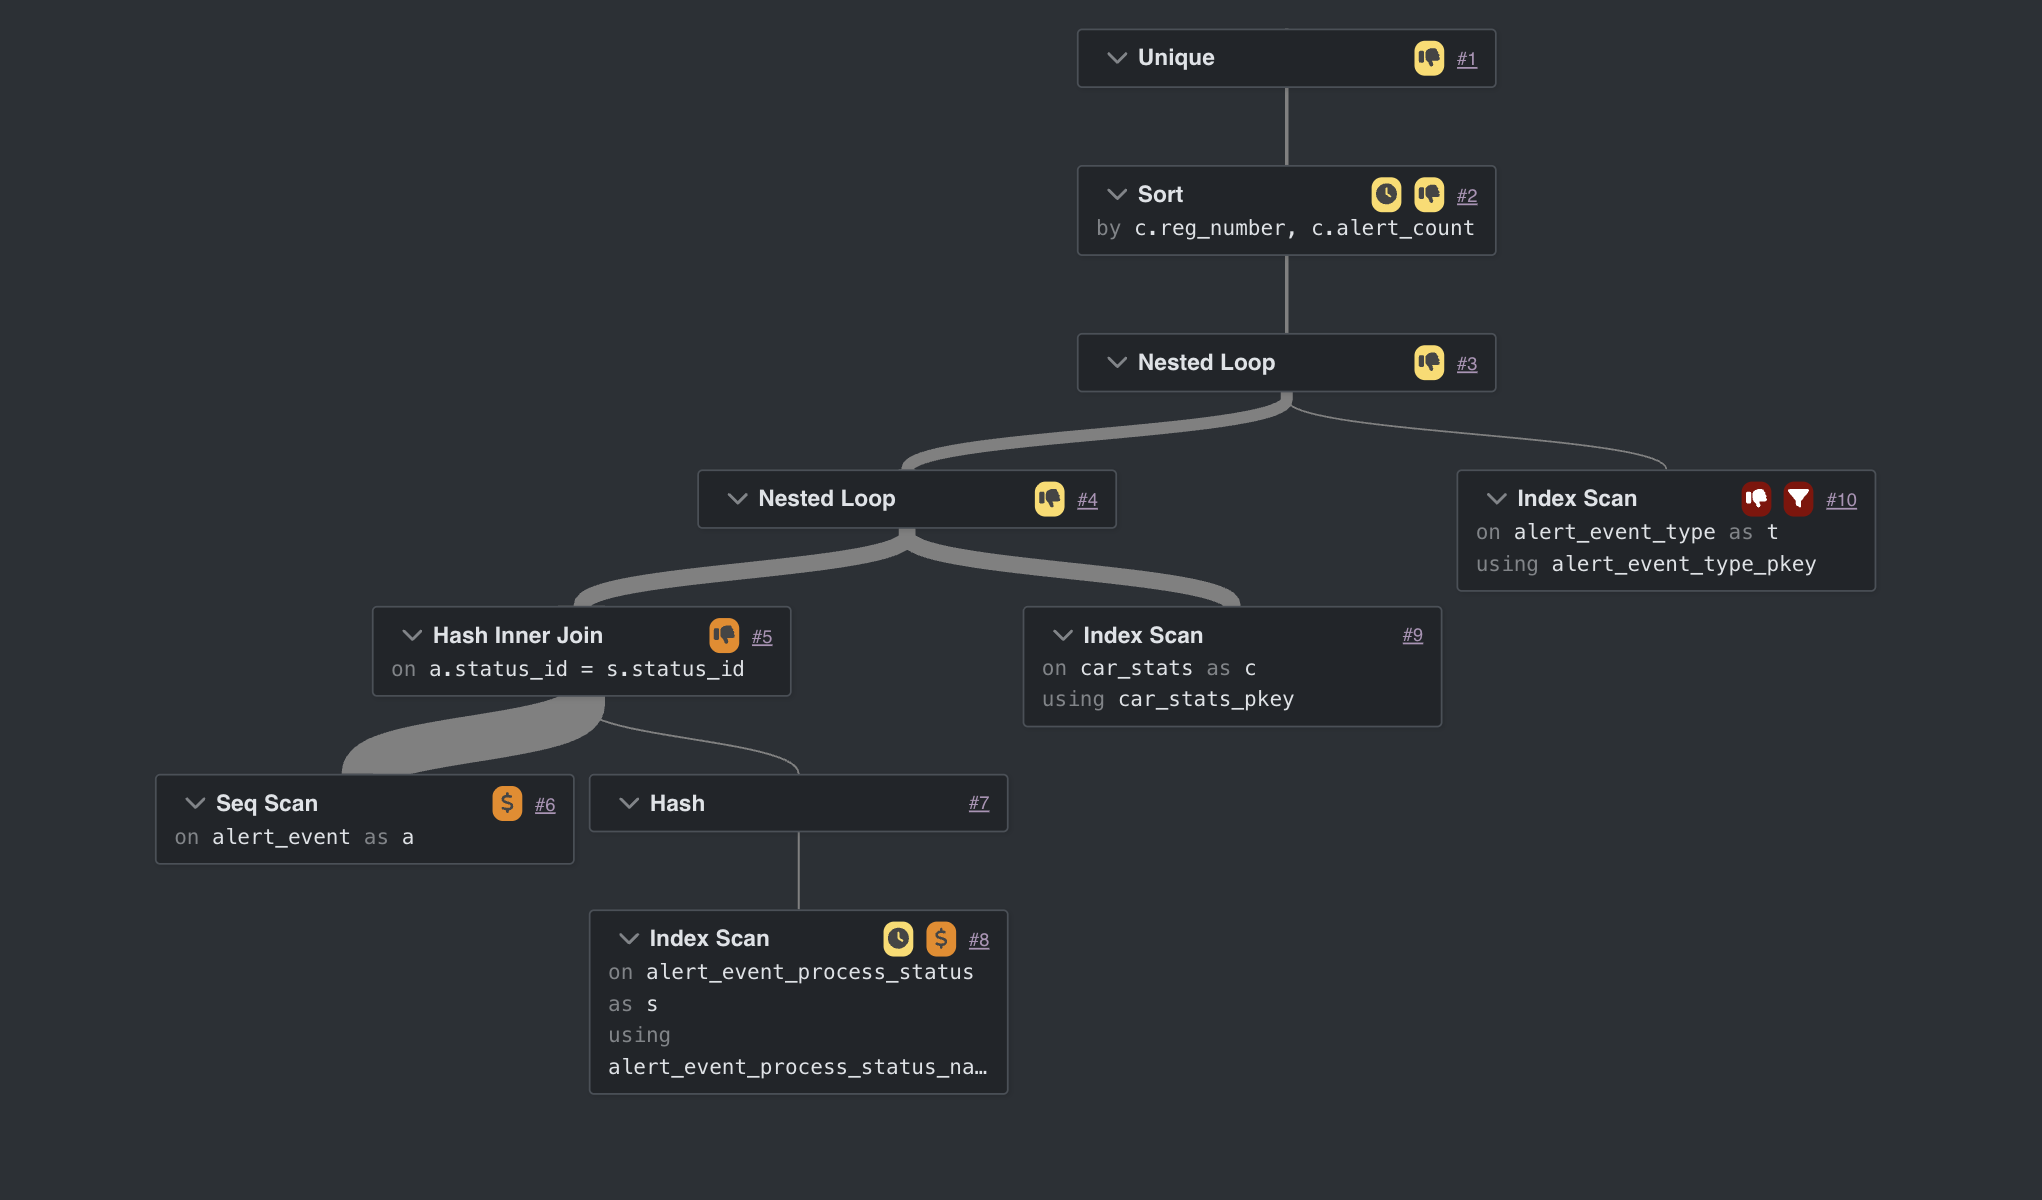
\includegraphics[width=0.85\linewidth]{myPhoto/hard_explain.png}
    \caption{Последовательность выполнения сложного запроса}
    \label{fig:hard_explain}
\end{figure}

\noindent Сначала последовательно читается таблица \textbf{alert\_event},
а по индексу находятся статусы обработки с именем «Новое». Эти таблицы
соединяются через Hash Join. Затем для каждого подходящего события по
первичному ключу находятся строка в \textbf{car\_stats} и его тип события.
В конце результат сортируется, а оператор \textbf{Unique} удаляет
повторяющиеся автомобили.

\noindent Реляционная формула запроса:
\[
\begin{aligned}
&\pi_{\text{reg\_number},\;\text{alert\_count}}
\Bigl( \\
&\quad\sigma_{
  \substack{
    \text{parking\_count}<18\;\wedge\;\text{s.name}=\text{«Новое»}\;\wedge;\text{t.name}=\text{«Потеря связи»}
  }
}\Bigl( \\
&\qquad\Bigl( \\
&\qquad\quad\text{car\_stats} \\
&\qquad\quad\bowtie_{\text{car\_id}}\;\text{alert\_event} \\
&\qquad\quad\bowtie_{\text{status\_id}}\;\text{alert\_event\_process\_status} \\
&\qquad\quad\bowtie_{\text{alert\_event\_type\_id}}\;\text{alert\_event\_type} \\
&\qquad\Bigr) \\
&\quad\Bigr) \\
&\Bigr)
\end{aligned}
\]

\newpage
% \subsection{Проверка доступа к представлению}

% В созданном представлении был проверен доступ на изменение данных. В данном представлении нельзя было сделать изменения, так как оно было создано при помощь GROUP BY. В качестве подтверждения был выполнен запрос на изменение данных в представлении, который выдал ошибку. Результат выполнения запроса представлен на листинге~\ref{fig:hard_query_result}.

% \begin{figure}[H]
%     \centering
%     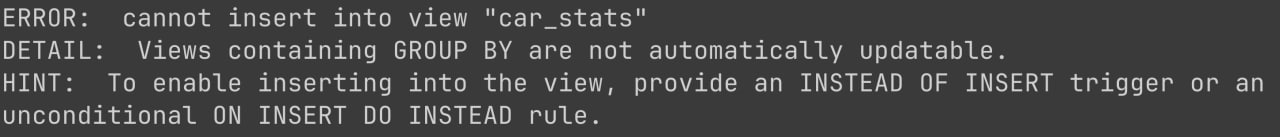
\includegraphics[width=0.8\linewidth]{myPhoto/avability.jpg}
%     \caption{Ошибки выдаваемые при попытке изменения данных в представлении}
%     \label{fig:hard_query_result}
% \end{figure}
